\documentclass[12pt, a4paper, oneside]{article}
\usepackage{fancyvrb,url}
\DefineVerbatimEnvironment{code}{Verbatim}{fontsize=\small}
\DefineVerbatimEnvironment{example}{Verbatim}{fontsize=\small}
\newcommand{\ignore}[1]{}
\usepackage[usenames]{color}
\usepackage{hyperref}
\usepackage{pxfonts}
\newsavebox{\spaceb}
\newsavebox{\tabb}
\savebox{\spaceb}[1ex]{~}
\savebox{\tabb}[4ex]{~}
\newcommand{\hsspace}{\usebox{\spaceb}}
\newcommand{\hstab}{\usebox{\tabb}}
\newcommand{\conceal}[1]{}

% turn of those nasty overfull and underfull hboxes
\hbadness=10000
\hfuzz=50pt

\usepackage{listings}
\usepackage{color}
\usepackage{textcomp}
\usepackage{parskip}
\usepackage{graphicx}
\definecolor{listinggray}{gray}{0.9}
\definecolor{lbcolor}{rgb}{1,1,1}
\lstset{
	backgroundcolor=\color{lbcolor},
	tabsize=4,
	rulecolor=,
	language=Haskell,
    upquote=true,
    aboveskip={1.5\baselineskip},
    columns=fixed,
    showstringspaces=false,
    extendedchars=true,
    breaklines=true,
    prebreak = \raisebox{0ex}[0ex][0ex]{\ensuremath{\hookleftarrow}},
    frame=none,
    showtabs=false,
    showspaces=false,
    showstringspaces=false,
    identifierstyle=\ttfamily,
	keywordstyle=\bfseries\ttfamily\color[rgb]{0,0,1},
	identifierstyle=\ttfamily,
	commentstyle=\color[rgb]{0.133,0.645,0.133},
	stringstyle=\ttfamily\color[rgb]{0.627,0.126,0.941},
	showstringspaces=false,
	basicstyle=\scriptsize,
	numberstyle=\footnotesize
}

\usepackage{bussproofs}
\usepackage{amssymb}
\usepackage{latexsym}

% This is the "centered" symbol
\def\fCenter{{\mbox{\Large$\rightarrow$}}}

% Optional to turn on the short abbreviations
\EnableBpAbbreviations

\begin{document}
(note this is a draft,I plan to change the actual source codes to psuedo-source, which hides the implementation choices like constructor names. And also apply proper typesetting and replace the images with actual latex code. I'll also move to generating documentation like UHC does)

\section{HML}
The type system implemented in this thesis is called HML, this section explains the finer details of the type system which is needed to understand the rest of this thesis.

\subsection{Types}

\begin{figure}[h!]
  \centering
    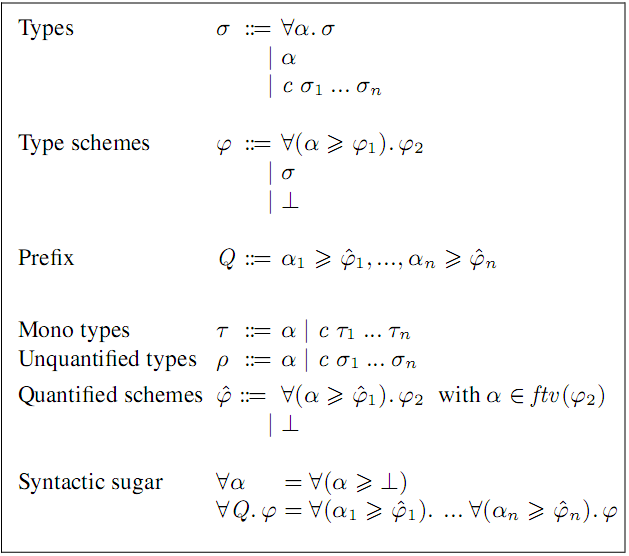
\includegraphics[width=0.8\textwidth]{types}
  \caption{HML Types}
\end{figure}

The types in HML are relatively simple. The first types in the figure are the SystemF ($\sigma$) types. You have the case for Quantification $\forall \alpha.\sigma$ which binds $\alpha$ in $\sigma$. The second case is the case for variable $\alpha$ and the last case is the case for constructors $c \sigma_1 \ldots \sigma_n$. The construct $\rightarrow$ is not treated any specially in this type system.

Type Schemes ($\varphi$) are the most important types in HML. It consist of the bottom $\bot$ type, which signifies undefined values. A type scheme can also consist of a systemF type $\sigma$ or be a quantified type. The form of the quantification is different than that of SystemF types. The quantification $\forall(\alpha \geq \varphi_1). \varphi_2$ should be interpreted as \emph{in the type $\varphi_2$ the variable $\alpha$ is bound by the quantification. The value of $\alpha$ can be any instantiation of the type $\varphi_1$}. These quantifications can be arbitrarily deep or long. e.g. $\forall(\alpha \geq \forall(\beta \geq \varphi_1). \varphi_3). \varphi_2$ which contains a deep nested type.

The next type is called the \emph{Prefix}. This is essentially a type environment where every variable $a_i$ is bound to the quantified type scheme $\hat{\varphi_i}$. The \emph{Prefix} cannot contain any \emph{trivial} types, which is to say, It can now contain any $\sigma$ types as a bound. Instead of creating a binding for such types inside the prefix a substitution is created instead. The subtitution environment will contain atleast those types that are not in bound in the prefix, or in other words, the domain of the subsitution environment $\theta$ and of the \emph{Prefix} are disjoint. Prefixes have a implicit ordering on them, the order of the elements in the prefix should always be the order in which they were introduced. This is important for a number of functions but also important for the right ordering of quantifications.

To express this limitation the Quantified schemes $\hat{\varphi}$ were created. However this shouldn't be viewed as a \emph{concrete} type, but rather a type synonym. The invariant on the Prefix is maintained by the functions that can extend the prefix. 

The Mono type $\tau$ and the Unquantified type $\rho$ types should be seen as a testable constraint and not real types. A type can be tested to see if it's a mono type, but no function actually generated a mono type. The following two types are purely syntactical sugar and don't actually exist. The first one simply states that the systemF quantification $\forall \alpha$ is equivallent to the type scheme quantification $\forall(\alpha \geq \bot)$, this is called an unconstrained bound. The second states that quantifying a type scheme with a Prefix means concatinating the types in the Prefix together. It's also important to note that every SystemF type can be represented as a flexible type, and vice-versa.

\subsection{Normal Form}
In order to easily compare types, they are usually converted to normal form first. This convertion si specified by:

\begin{figure}[h!]
  \centering
    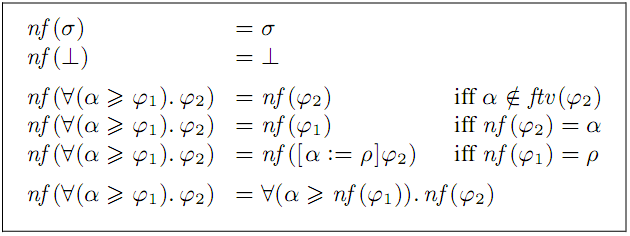
\includegraphics[width=0.8\textwidth]{nf}
  \caption{Normal form conversion}
\end{figure}

\subsection{Utility functions}
There are a number of simple utility functions to make things easier. These all operate on the Prefix $Q$ and all keep the invariant placed on $Q$.

\begin{figure}[h!]
  \centering
    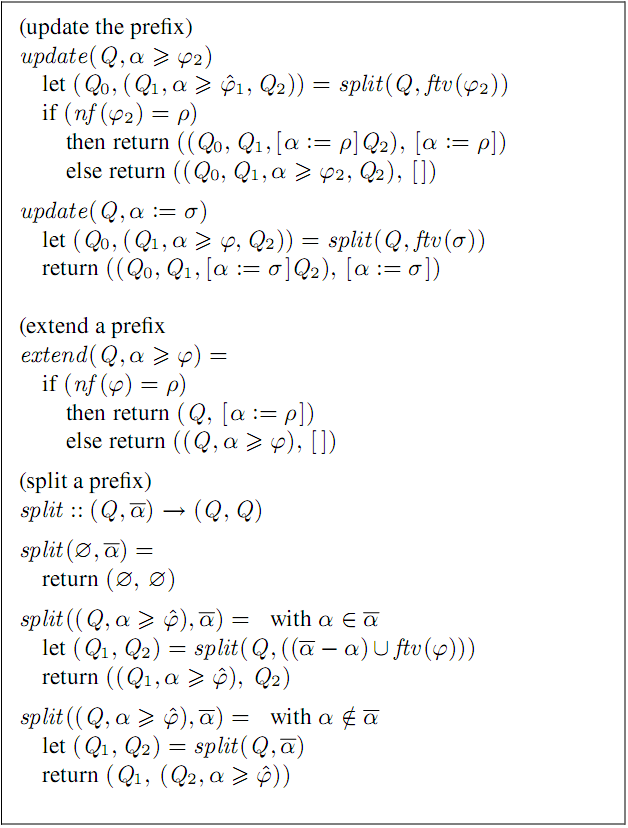
\includegraphics[width=0.8\textwidth]{utils}
  \caption{Utility functions}
\end{figure}

\subsubsection{update function}
The update functions updates a prefix with a new binding or updates an existing binding.
$update(Q, \alpha \geq \varphi_2)$ updates the binding for $\alpha$ in $Q$. First $Q$ is split based on the free variables of $\varphi_2$. This is a form of scoping and in the case that $\alpha \in ftv(\varphi_2)$ is prevents a possible infinite expansion(by repeated calls to update). The existing binding to $\alpha$ in the Prefix is removed leaving 3 sub prefixes. The prefixes $Q_0$ and $Q_0$ have no further influence on the operations, but the Prefix $Q_2$ can contain references to $\alpha$. Remember the invariant on Q and that prefixed when desugared follow eachother. For example $[(\alpha \geq \bot), (\beta \geq (\forall(\gamma \geq \bot).\alpha \rightarrow \gamma))]$ is a valid type and would be unfolded to $\forall(\alpha \geq \bot). \forall(\beta \geq (\forall(\gamma \geq \bot).\alpha \rightarrow \gamma)). \beta$ for instance.

The first check is to see if the normal form of $\varphi_2$ is a unquantified type. This check preserves the invariant that no trivial bounds (e.g. unquantified type) can enter the environment. If the type is unquantified, the substitution $[\alpha := \sigma]$ is applied to $Q_2$ since there is no longer any binding for $\alpha$ in the prefix, the result of the substitution is concatinated with $Q_0$ and $Q_1$ in the order specified to retain the invariant. Along with the new Prefix the substitution is returned so that any other type can also be updated. If the type is not a unquantified type a new binding $\alpha \geq \varphi_2$ is put in the environment in the same place as the old one was removed. This function also illustrates that $\varphi$ and $\hat{\varphi}$ are the same types.

$update(Q, \alpha := \sigma)$ is the same as $update(Q, \alpha \geq \varphi_2)$ when $nf(\varphi_2)$ is a unquantified type.

\subsubsection{extend}
Extends attemps to extend the Prefix with a new entry, just as update is does so only if the normal form of the bound is not a unquantified type. If that is not the case a substitution is returned instead.

\subsubsection{split}
The split function is the most trivial of the three, It just splits the prefix in 2. The first containing all the bindings where the variable is an element of the variable list given and the second with the those that are not. The ordering is broken, but inside the two Prefixes the invariant still holds. Because of the way split is used (e.g. always on the ftv list of a binding we're updating) the invariant would still hold after concatinating the two prefixes back together.

\subsection{Inferrence}

The inferrence algorithem is pretty self explanatory. The difference with the standard Hindley-Milner inferrence is that an extra environment $Q$ (the Prefix) is also passed along. The extend calls are how we insert a new binding inside the Prefix. A type is always quantified, either in the Prefix $Q$ or in the type itself. It will be elaborated on later when the EH implementation of it is presented.

\begin{figure}[h!]
  \centering
    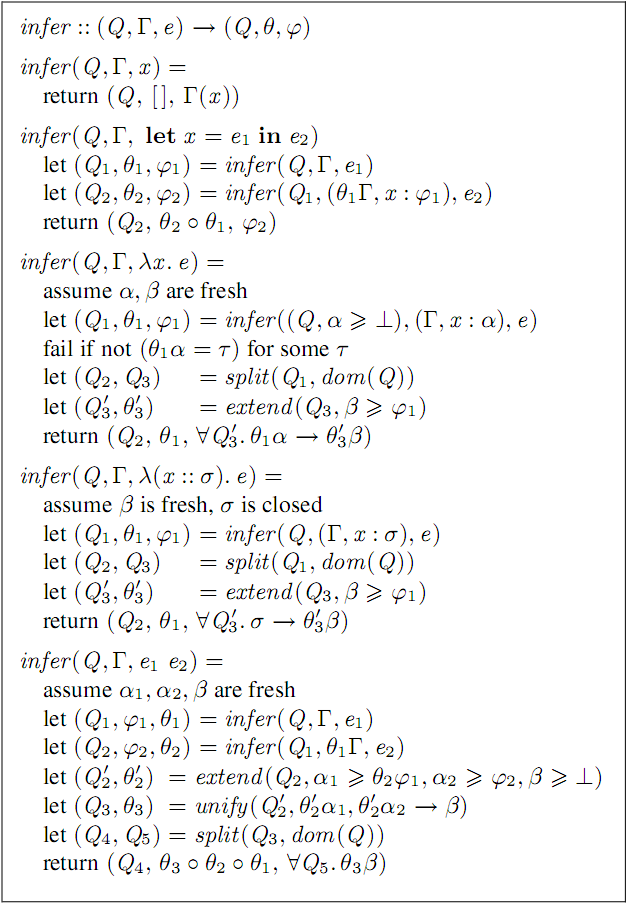
\includegraphics[width=0.8\textwidth]{infer}
  \caption{Inferrence algorithm}
\end{figure}

It is important to note that the result of the inferrence will always be the desugared types, since the syntactical sugar is not an actual type.

\subsection{Unification}

\begin{figure}[h!]
  \centering
    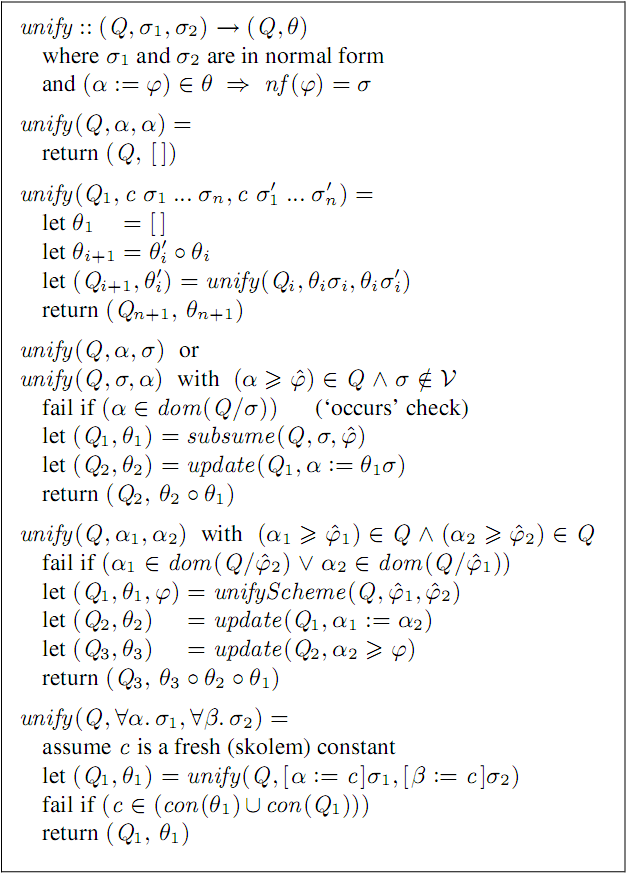
\includegraphics[width=0.8\textwidth]{unify}
  \caption{Unification algorithm}
\end{figure}

The unification function will be elaborated on in the implementation section, just as the inferrence algorithm. Here we would like to point out that it uses a mix of SystemF types $\sigma$ and flexible types $\varphi$. In particulair we beleive this is not needed and it would be much nicer to only use one of the two typee. Since a systemF type can always be expressed in a flexible type we will show a version of unify that uses only flexible types.

The last case if never used during normal unification. It's only used when you specifically want to unifify two quantified systemF types. for instance when checking a type signature given by a user with a inferred type.

$\alpha \in dom(Q/\hat{\varphi})$ should be seen as a reachability test. It means formally that $\alpha \in dom(Q/\hat{\varphi})$ if and only if $Q = (Q_1, a \geq \hat{\varphi_1}, Q_2)$ and $\alpha \in ftv(\forall Q_2. \varphi)$. As an example $dom((\gamma \geq \bot, \beta \geq \forall \delta. \delta \rightarrow \gamma)/(\forall \alpha. \alpha \rightarrow \beta))$ is $\{\beta, \gamma\}$ because even though $\gamma$ is not directly reachable from the type is is reachable by $\beta$.

\subsection{Instantiation}
The next two functions are instantiation and scheme unification.

\begin{figure}[h!]
  \centering
    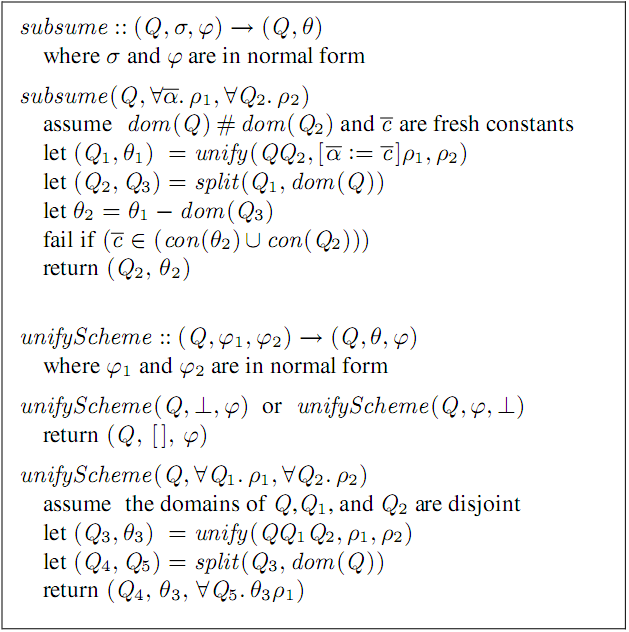
\includegraphics[width=0.8\textwidth]{subsume}
  \caption{subsume \& unifyScheme}
\end{figure}

Instantiation is just your standard instantiation, We're tying to instantiate the first type with the second type. In order to assure that we don't instantiate quantified variables we skolemize them and call unify again. Afterwards we return the a the updated bindings for the entried that were originally already in the Prefixed passed to instantiate, they now contain the bindings needed to instantiate $\rho_1$ to $\rho_2$. But since simple bounds can't be in the prefix, we also need to return the scoped substitutions. We also scope the substitutions so that skolem variables don't escape from instantiation since they hold no intrinsic value and would prevent further unification. This function is what handles higher-rank types.

However a very important case is missing from the given specification, which is when we try to instantiate a type with $\bot$. Since instantiation always succeeds when instantiating to $\bot$ we should always return $(Q, [])$ for calls to $subsume(Q, \sigma, \bot)$.

UnifyScheme is used to unify two flexible types. It returns aside from a new Prefix and substitution environment also the most general type $\varphi$ that describes both $\rho_1$ and $\rho_2$. In other words, using the Prefix $Q$ and the substitutions $\theta$, $\rho_1$ and $\rho_2$ can be instantiated to $\varphi$.

\subsection{Typing rules}
The type rules in HML are almost the same as the ones in Hindley-Milner, except that in the presence of \textit{flexible} types the Instantiation rule is slightly different and every rule now gets an explicit \textit{Prefix}. 

\begin{prooftree}
		\AxiomC{$x : \varphi \in \Gamma$}
	\LeftLabel{Var:\quad}
		\UnaryInfC{$Q,\Gamma\vdash x : \varphi$}
\end{prooftree}

The var rule is still very straight forward, if there is a binding for x in the environment $\Gamma$ with the type $\varphi$ then return the type of $\varphi$ for x under the same environment $\Gamma$ and prefix $Q$.

\begin{prooftree}
		\AxiomC{$Q,\Gamma\vdash e : \varphi_1 \quad Q \vdash \varphi_1 \sqsubset \varphi_2$}
	\LeftLabel{Inst:\quad}
		\UnaryInfC{$Q,\Gamma\vdash e : \varphi_2$}
\end{prooftree}

The instantiation rule states that we can always use a instance of a type under the prefix $Q$ as the type of the expression. This instance of relation is denote by the $\sqsubset$ relation above which states that $\varphi_2$ is an instance of $\varphi_1$ under the prefix $Q$

\begin{prooftree}
		\AxiomC{$(Q, \alpha \geq \hat{\varphi}_1), \Gamma \vdash e : \varphi_2 \quad \alpha \notin ftv(\Gamma)$}
	\LeftLabel{Gen:\quad}
		\UnaryInfC{$Q,\Gamma \vdash e : \forall(\alpha \geq \hat{\varphi}_1) . \varphi_2$}
\end{prooftree}

The generalization rule generalizes a type by moving it's bounds out from the prefix $Q$ into the type $\varphi$.

\begin{prooftree}
		\AxiomC{$Q,\Gamma \vdash e_1 : \sigma_2 \rightarrow \sigma \quad Q,\Gamma \vdash e_2 : \sigma_2$}
	\LeftLabel{App:\quad}
		\UnaryInfC{$Q,\Gamma \vdash e_1 \hspace{3pt} e_2 : \sigma$}
\end{prooftree}

The application rule is the standard application rule over types. It requires that the type of $e_2$ be equal to the type of the argument of $e_1$. Note that this ranges over type and not typeschemes.

\begin{prooftree}
		\AxiomC{$Q,\Gamma \vdash e_1 : \varphi_1 \quad Q,(\Gamma, x : \varphi_1) \vdash e_2 : \varphi_2$}
	\LeftLabel{Let:\quad}
		\UnaryInfC{$Q,\Gamma \vdash \textbf{Let} \hspace{3pt} x = e_1 \hspace{3pt} \textbf{in} \hspace{3pt} e_2 : \varphi_2$}
\end{prooftree}

The Let rule is pretty straight forward, given an expression $e_1$ with type $\varphi_1$ and a variable $x$ which in the environment $\Gamma$ has the same type $\varphi_1$ and an expression $e_2$ with type $\varphi_2$ we can create a let binding \textbf{Let} x = $e_1$ \textbf{in} $e_2$.

\begin{prooftree}
		\AxiomC{$Q, (\Gamma, x : \tau) \vdash e : \sigma$}
	\LeftLabel{Fun:\quad}
		\UnaryInfC{$Q, \Gamma \vdash \lambda x. e : \tau \rightarrow \sigma$}
\end{prooftree}

The Fun rule restricts the type of the parameter to a monomorphic type $\tau$ in order to avoid having to guess polymorphic types. This does not mean that a polymorphic type can not be infered since the type schemes are hidden in the prefix $Q$.

\begin{prooftree}
		\AxiomC{$Q, (\Gamma, x : \sigma_1) \vdash e : \sigma_2$}
	\LeftLabel{Fun-Ann:\quad}
		\UnaryInfC{$Q, \Gamma \vdash \lambda(x :: \sigma_1). e : \sigma_1 \rightarrow \sigma_2$}
\end{prooftree}

The Function Annotation rule is used to provide a mechanism to explicitly annotate abstraction variables with a (possibly) polymorphic type. Like annotation of the \textit{push} example above with the needed higher-rank type.

In particular the \textit{FUN} rule for lambda expressions restrict the type of the parameters to be a mono type $\tau$ since any scheme on the mono type is in the Prefix $Q$, this is the secrete behind HML.

\section{Modifications to HML}
The implementation of HML differes somewhat compared to textbook HML\cite{HML}. During implementation of the algorithm we realised that internally it used both flexible types and SystemF types. This introduces a number of differences between the textbook implementation and the version we implemented.

$<$insert figure containing full algorithm here$>$

\subsection{Promotions}
We wanted to limit the amount that SystemF types were being used and promote more usage of flexible types during unification.
This is accomplished by modifying the \textit{extend} function, which is the only way to introduce a new type binding in the \textit{Prefix}. This function as mentioned before also enforces the invariant that no \textit{simple} bounds can enter the environment. These are instead returned as a substitution;

\begin{lstlisting}
extend :: (Prefix, Scheme) -> (Prefix, Env)
extend (q, (Scheme_Simple var phi))
 = let p = nf phi
   in case isUnQualTy p of
        True  -> (q, [(var, p)])
        _     -> (q++[TyIndex_Group var (promote phi)], [])
\end{lstlisting}

The only difference between this and the described function in the HML specification is that upon adding the type to the \textit{Prefix} it is first \textit{promoted} by the \textbf{Promote} function.

\begin{lstlisting}
promote :: TyScheme -> TyQuantifiedScheme
promote TyScheme_Bottom 
  = TyScheme_Bottom
promote (TyScheme_Quant (Scheme_Simple nm ty) ty') 
  = TyScheme_Quant (Scheme_Simple nm (promote ty)) ty'
promote (TyScheme_SystemF x)                   
  = embedF x
\end{lstlisting}

Implementing promote is pretty straight forward. If we find a $\bot$ value we just ignore it, if we find a type scheme we just have to check in it's bounds to make sure it doesn't contain a SystemF type, and if we find a SystemF type we convert it to a flexible type using \textit{embedF}.

\begin{lstlisting}
embedF :: TyExpr -> TyScheme
embedF = embed id
 where embed :: (TyScheme -> TyScheme) -> TyExpr -> TyScheme
       embed val (TyExpr_Parens     s) = embed val s
       embed val (TyExpr_Quant  _ a t) = let e = TyScheme_Quant (Scheme_Simple a TyScheme_Bottom)
                                         in  embed (val . e) t
       embed val e                     = val (TyScheme_SystemF e)
\end{lstlisting}

\textit{embedF} works by stripping every outter $\forall$-quantifiers and replacing them with type schemes instead. We only replace the outter quantifiers which means that the only $\forall$s still in the type would be those of higher rank types.

When confronted during unification with two quantified SystemF types the \textit{classic} implementation it proceeded by skolemizing both types and recursively call unification. If we were to remove the usage of SystemF types by unification this case would no longer be needed. The actual comparison is already being done by \textit{instantiation} (subsume) where we would still atmost have one quantified SystemF type. 

This SystemF type in \textit{subsume} can also be removed, but that would complicate both \textit{embedF} and \textit{subsume}. If we were to do it the required changes would be to change embedF to:

\begin{lstlisting}
embedF :: TyExpr -> Int -> TyScheme
embedF e = uncurry ($) . second (TyScheme_SystemF . fst) . embed False e
 where embed :: Bool -> TyExpr -> Int -> (TyScheme -> TyScheme, (TyExpr, Int))
       embed b (TyExpr_Parens     s) i = if b 
                                          then let (f1, (e, i')) = embed False s i
                                                   (var, ires)   = freshT "t" i'
                                                   f2            = TyScheme_Quant (Scheme_Simple var (f1 $ TyScheme_SystemF e))
                                               in (f2, (TyExpr_Var var, ires))
                                          else second (first TyExpr_Parens) (embed b s i)
       embed b (TyExpr_Quant  _ a t) i = let e = TyScheme_Quant (Scheme_Simple a TyScheme_Bottom)
                                         in  first (e.) $ embed b t i
       embed b (TyExpr_Forall _ v t) i = let e = foldl' (.) id [ TyScheme_Quant (Scheme_Simple a TyScheme_Bottom) | a <- v ] 
                                         in  first (e.) $ embed b t i
       embed b (TyExpr_AppTop     x) i = let (f, (e, i')) = embed b x i
                                         in  (f, (TyExpr_AppTop e, i'))
       embed _ (TyExpr_App      f x) i = let (f1, (e1, i1)) = embed True f i
                                             (f2, (e2, i2)) = embed True x i1
                                         in  (f2 . f1, (TyExpr_App e1 e2, i2))
       embed _ e                     i = (id, (e, i))
\end{lstlisting}

where \textit{first} and \textit{second} are arrow functions. In this context \emph{first f} applies f to the first element in the tuple and \emph{second} to the second element respectively. \emph{freshT} generates a fresh variable using the given template \emph{"t"} in this case and a starting point.

The reason we need to generate a fresh variable is that a type scheme is not valid within a systemF type. As an example, the type $\forall a. \forall b. (\forall c. c \rightarrow Int) \rightarrow a \rightarrow b$ would become the following flexible type: $(a \geq \bot). (b \geq \bot). (t1 \geq (c >= \bot). c \rightarrow Int). t1 \rightarrow a \rightarrow b$.

The next objective is to modify \emph{subsume} to take two flexibly types as argument and to skolemize the variables of the first type where they're bound to a $\bot$. e.g. in the example above only a and b should be skolemized. This is because skolemization is done on bounded quantifiers, and \emph{t1} is not a $\forall$ in systemF but a type.

\subsection{Renaming}
When typechecking an expression such as (id id) the environment would return the same type for both occurences of id, this is logical since they are the same values. However because they use the same type variables unification will get confused and accidently apply substitution to both types.

Both types are entered into the Prefix, however, eventually when both are inspected the same binding (e.g. $(a \geq \bot)$) will be put in the prefix. While there are two occurences, there's nothing that distinguishes between them. Because of the ordering inside the Prefix, any actions executed which was intended to be executed on the second entry is only applied to the first.

To prevent this, we explicitly $\alpha$-rename types before we add them to the Prefix. this also ensures that all type variables are unique. We must also store the $\alpha$-renaming substitution and include it in the final substitution mappings returned from unification. This becomes apparent if we look at the simple example of

\begin{lstlisting}
op :: (Int -> t) -> t
op = \x -> x 1
\end{lstlisting}

When the variable \emph{x} is introduced in the $\lambda$-abstraction it is given a type \emph{a}. During unification the type of \emph{x} is renamed to \emph{b} and the type of \emph{b} is later inferred to be (Int $\rightarrow$ t) but in the $\lambda$ \emph{x} is still bound to \emph{a}, which is why the renaming substitution (\emph{a}, \emph{b}) should be returned.

\subsection{Prefix scoping}
Because we now produce very deeply embedded types from the type checker, in order to get scoping of the type variables correct a few changes had to be made.

\subsubsection{Prefix Domain}
The domain of a prefix $\mathcal{Q}$ is $\{a_1\ldots a_n\}$ where $\{(a_1 \geq \ldots) , \ldots , (a_n \geq \ldots)\}$. A consequence of having mostly flexible types during unification is that deeply nested type schemes can be created (most are only 2 levels deep however). This is a problem for the correct scoping of types. Consider the example \emph{map id} where $id :: (a \geq (b \geq \bot). b \rightarrow b). a$

The type returned would be $[b] \rightarrow [b]$ with in the prefix the binding for \emph{b} $(b \geq \bot)$ and not $[a] \rightarrow [a]$. When we generalise on the result of unification we do so based on the \emph{domain} of the original prefix passed to the call which in this case would be just {a}. 

What we end up determining for \emph{map id} is thus improperly scoped since \emph{b} was never in the original domain. For this reason we change the definition of \emph{domain} to also take into account the recursive nature of prefixes;

\begin{lstlisting}
instance Domain TyIndex where
  domain   (TyIndex_Group a b) = a : binds b
    where binds :: TyScheme -> [HsName]
          binds (TyScheme_Forall a _) = a
          binds (TyScheme_Quant a b ) = domain a ++ binds b
          binds                     _ = []
\end{lstlisting}

The domain for \emph{id} now returns {a, b} which now allows us to properly apply generalisation.

\subsubsection{Type split}
When typing types such as that of the compose function \emph{(f (g x))} the type of \emph{f} depends on the type of \emph{g} which in turn depends on the type of \emph{x} alot of information is "hidden" in the recursive prefixes returned by infer. To properly account for these we introduce the type rule \textbf{Scope}

\begin{prooftree}
		\AxiomC{$Q,\Gamma\vdash e : \forall Q_1.\varphi$}
	\LeftLabel{Scope:\quad}
		\UnaryInfC{$Q Q_1,\Gamma\vdash e : \varphi$}
\end{prooftree}

This rule moves the bounds from the type itself into the environment. Because a type is either fully quantified or bound by the environment this rule is sound and thus safe to perform.

\subsection{Desugaring}
At the end of every \emph{infer} step, we generalise the type and return it. This is done using the syntax $\forall Q. \varphi$ which is syntactical sugar for the unfolding introduced in the previous chapter.

However we take this opportunity to simplify the type a bit. Instead of just returning the unrolled type we redefine the \emph{desugar} step to also perform a partial convertion. 

\begin{quotation}
\noindent ptype($\varphi$) = ft($\varphi$)\\
\indent\indent where \\
          \indent\indent\indent ft($\forall(\alpha \geq \forall Q. \rho). \varphi$) = ft($\forall Q.[\alpha \Coloneqq \rho]\varphi $)\\
          \indent\indent\indent ft(x)\indent\indent\indent\indent  = x\\
\end{quotation}
This will only be done at the very end, and is done to remove superfluous bindings such as the one seen in the \emph{id} example and to simplify the type we return to the user. The resulting type has the added benefit of also being in normal form.

While this isn't strictly needed, the alternative would be to just use the classical desugaring method, but then we'd have to complicate lookups of bindings in the Prefix and also the removal of a binding;

Given a Prefix $(a \geq (b \geq \bot). b \rightarrow b)$ we end up at the situation where if we were to lookup a, we'd find a flexible type which is bound by a variable \emph{b}. We continue using this result until at somepoint we lookup what \emph{b} is supposed to be and we remove it. But removing \emph{b} in this case would also mean removing \emph{a} and any parent of \
\subsection{Normal Form Checks}
In \textit{unifyScheme} and \textit{subsume} there are checks to see whether the types given as an argument to the functions are in normal form. This is now no longer the case. Because the types are now more recursive than before they are now no longer always in normal form, for instance \emph{$(a \geq \bot).a$} whose normal form is $\bot$ is not a valid argument to that function.

We now relax these restriction and allow any type to be passed to the functions, but because these functions \emph{compare} types we now perform explicitly convert the types to normal forms instead. This keeps these functions simple. If we were to not force the types to normal form we would have to perform extra lookups. Instantiation of \emph{b} and \emph{$(a \geq \bot).a$} would have to lookup what \emph{a} is before determening that \emph{a} is bound by $\bot$ and is thus fully polymorphic, in which case instantiation of \emph{b} is complete.
\section{Algorithm in terms of EH}
The algorithm detailed by the HML paper was given in terms of a very small $\lambda$-calculus which includes Let bindings. In order to implement it had to be \emph{scaled} up in terms of EH.
\begin{thebibliography}{9}
\bibitem{UHC}
  Utrecht Haskell Compiler Structure
  \emph{Structure Documentation}
   \url{http://www.cs.uu.nl/wiki/bin/view/Ehc/EhcStructureDocumentation}
\bibitem{uuagc}
  UUAGC
  \emph{"Utrecht Attribute Grammar System"}
   \url{http://www.cs.uu.nl/wiki/bin/view/HUT/AttributeGrammarSystem}
\bibitem{ruler-front}
  Arie Middelkoop, Atze Dijkstra, S.Doatse Swierstra
  \emph{Iterative Type Inference with Attribute Grammars}
  Utrecht University
\bibitem{Guesses}
  Arie Middelkoop, Atze Dijkstra, S.Doatse Swierstra, Lucilia Camarao de Figueiredo
  \emph{Controlling Non-Determinism in Type rules using First-Class Guessing}
  Utrecht University, Universidade Federal de Ouro Preto
\bibitem{Ruler}
  Atze Dijkstra, S. Doaitse Swierstra 
  \emph{Ruler: Programming Type Rules}
  LNCS FLOPS 2006 proceedings of FLOPS 2006
\bibitem{Monads}
  Arie Middelkoop, Atze Dijkstra, S.Doatse Swierstra
  \emph{Factoring Type Rules Into Aspects}
  Utrecht University
\bibitem{EH}
  Atze Dijkstra
  \emph{Stepping through Haskell}
  ISBN 90-393-4070-6
\bibitem{outsidein}
  Dimitrios Vytiniotis, Simon Peyton-Jones, Tom Schrijvers, Martin Sulzann
  \emph{Modular type inference with local assumptions}
  Microsoft Research, Katholieke Universiteit Leuven, Informatik Consulting Systems AG.
  Submitted to Journal of Functional Programming.
\bibitem{boring}
  Simon Peyton Jones, Dimitrios Vytiniotis, Stephanie Welrich and Mark Shields
  \emph{Practical type inference for arbitrary-rank types}
  Microsoft Research, University of Pennsylvania, Microsoft
\bibitem{FPH}
  Dimitrios Vytiniotis, Stephanie Weirich and Simon Peyton Jones
  \emph{FPH: First-class Polymorphism for Haskell}
  University of Pennsylvania and Microsoft Research
\bibitem{HML}
  Daan Leijen
  \emph{Robust type inference for first-class polymorphism}
  Microsoft Research
\bibitem{odesky}
  Martin Odersky and Konstantin Laufer
  \emph{Putting Type Annotations to Work}
  University of Karlsruhe and Loyola University Chicago
\bibitem{pierce}
  Benjamin C. Pierce and David N. Turner
  \emph{Local Type Inference}
  Indiana University and Technology Transfer Center
\end{thebibliography}
\end{document}
